\lecture{28}{12. Januar 2026}{2025 ReExam}

\begin{problemwithimage}{e2025r1}{1}
  Consider the simple truss structure, where the joints are numbered progressively from $A$ to $F$ and the length parameter $L$ is equal to \qty{1,0}{\m}.
  The truss is supported by a smooth pin at $C$ and a roller at $D$.
  Two forces of magnitude $F_1 = \qty{75}{\kN}$ and $F_2 = \qty{212,1}{\kN}$ are applied at joints $A$ and $F$, respectively.
  The direction of these two forces is as indicated on the figure.

  \begin{itemize}
    \item[Q1.1] Identify all the zero-force members in the truss structure
    \item[Q1.2] Determine whether the structure is statically determinate.
    \item[Q1.3] Find the reaction forces at $C$ and at $D$.
    \item[Q1.4] Use the method of joints to find the force in member $CE$.
  \end{itemize}

  The truss members are slender bars made of titanium (Young's modulus \qty{120}{\GPa}), with cross-sectional area $A = \qty{625}{\mm^2}$.

  \begin{itemize}
    \item[Q1.5] Calculate the length variation of member $CE$ due to the forces applied to the truss.
  \end{itemize}
\end{problemwithimage}

\begin{derivation}
  \begin{itemize}
    \item[Q1.1] We immediately realize that $AB$ must necessarily be a zero-force member as it is the only member supplying a force in the $x$ direction at $A$. This is confirmed to be the only zero force member by a truss analysis in MDSolids as shown on \Cref{fig:e2025r1t}.

      \begin{figure} [ht]
        \centering
        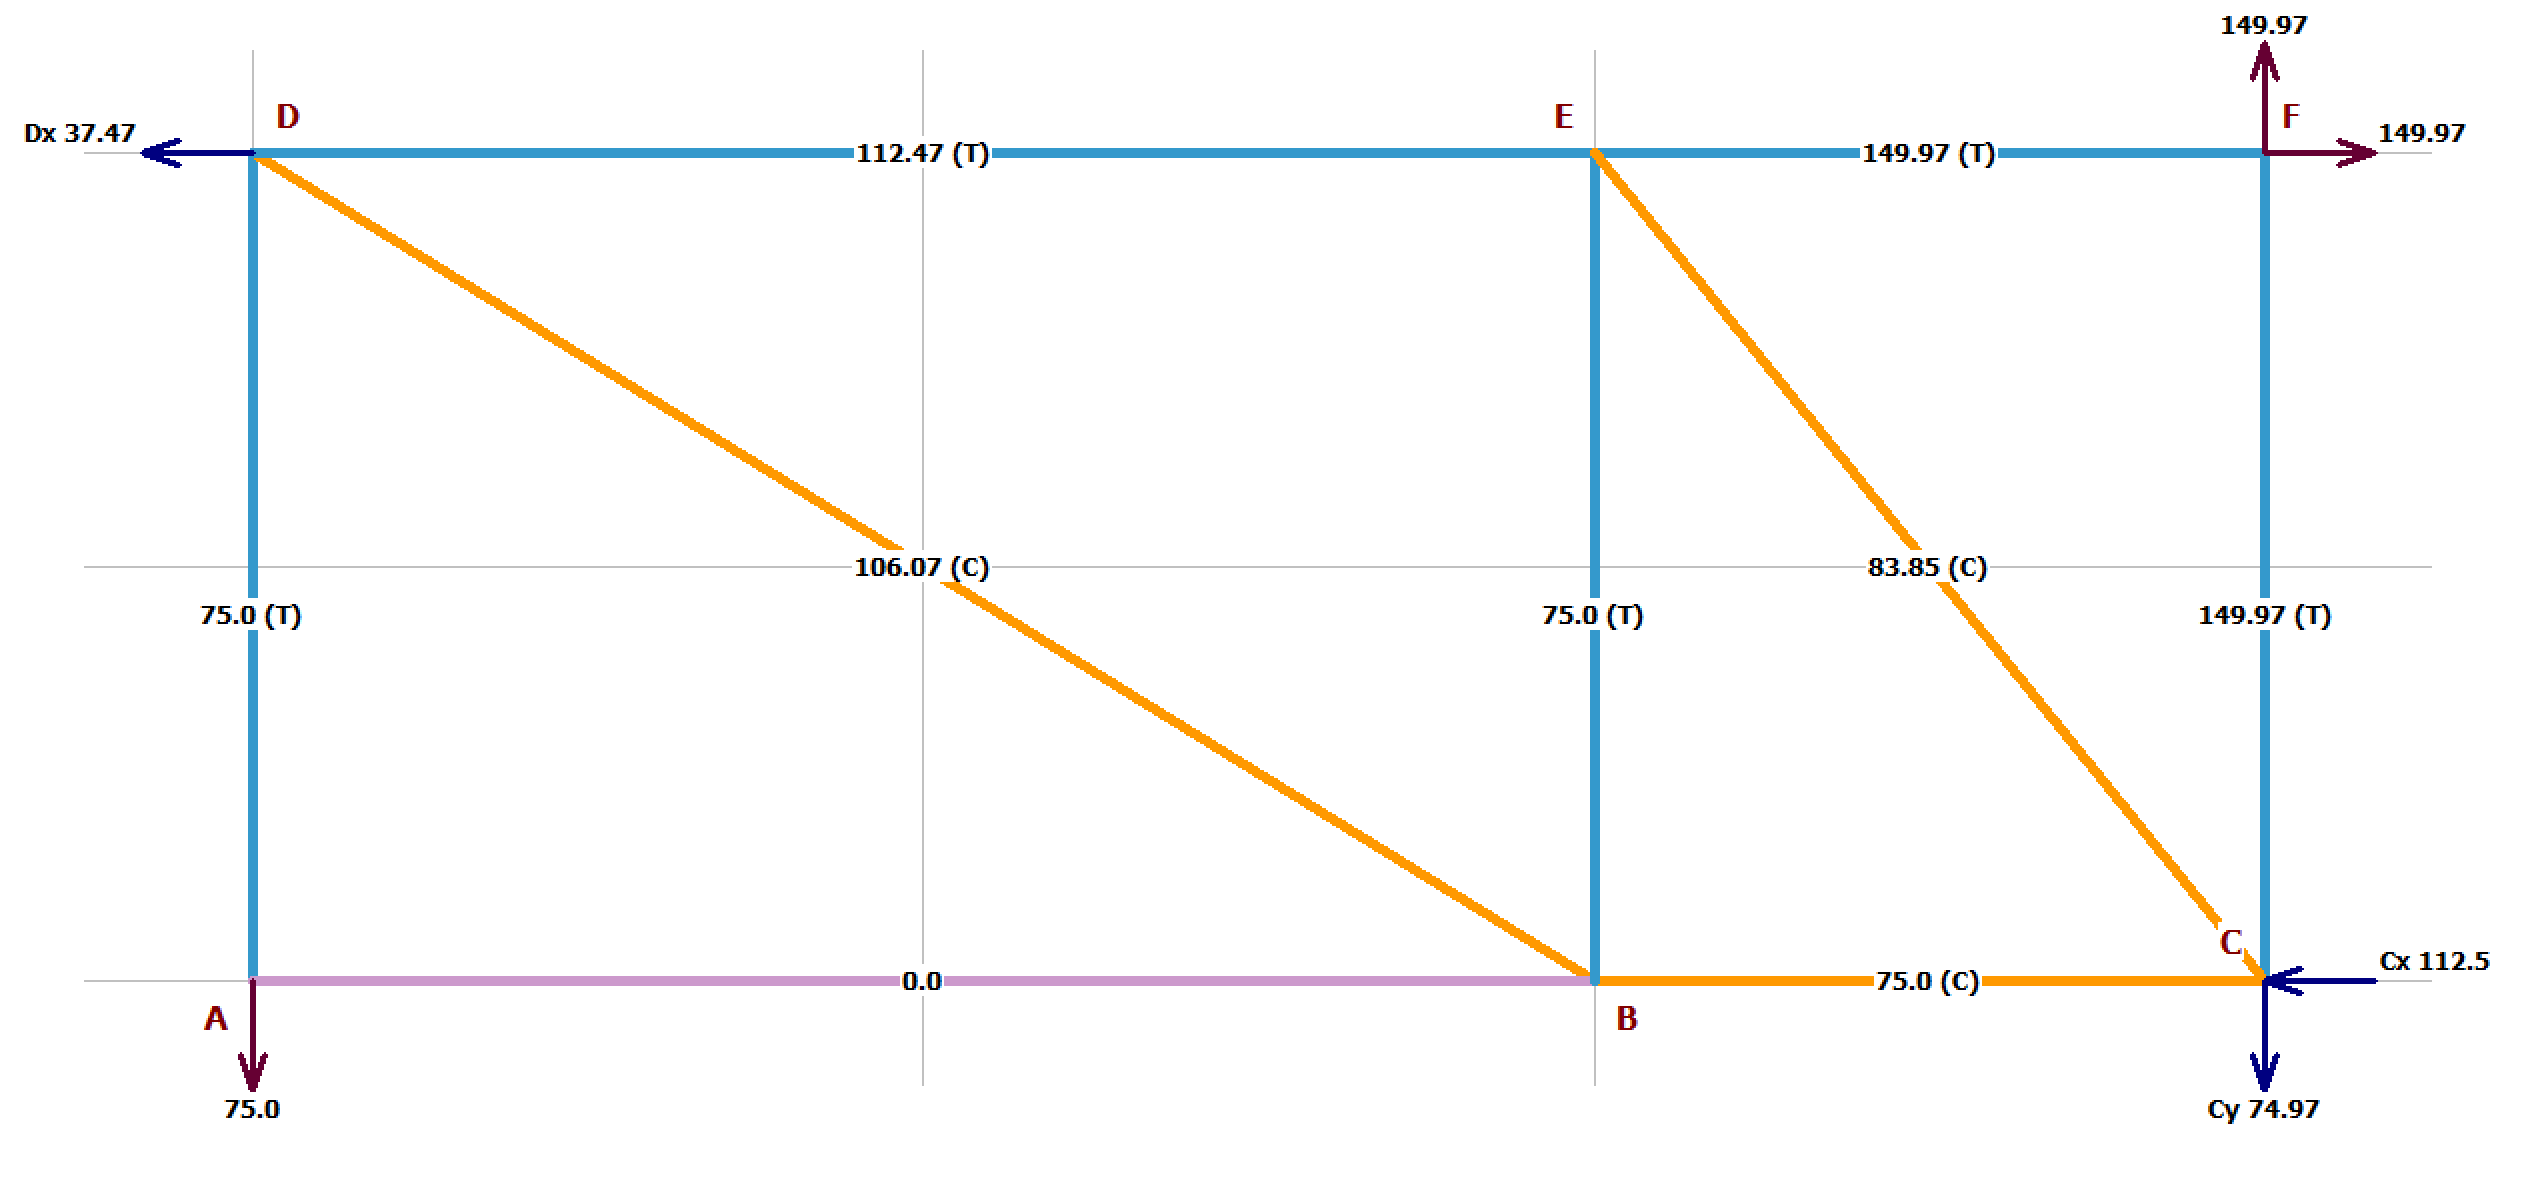
\includegraphics[width=0.8\linewidth]{./figures/e2025r1t.png}
        \caption{Truss analysis in MDSolids}
        \label{fig:e2025r1t}
      \end{figure}

    \item[Q1.2] We know that for a statically determinate truss the following equation holds:
      \begin{equation*}
        n_{\mathrm{member}} + n_{\mathrm{reactions}} = 2n_{\mathrm{joints}}
      .\end{equation*}
      Plugging in numbers (and remembering that $C$ supplies two reactions) we get:
      \begin{equation*}
        9 + 3 = 2 \cdot 6 = 12 
      .\end{equation*}
      which means the structure is statically determinate.

    \item[Q1.3] We need to find the reactions $D_x$, $C_x$ and $C_y$. 
      Using a force equilibrium in the $y$ direction we find $C_y$ as:
      \begin{align*}
        \sum F_y &= 0 \\
        - \qty{75}{\kN} + C_y + \qty{212,1}{\kN} \cdot \sin \ang{45} &= 0 \\
        C_y &= \qty{75}{\kN} - \qty{212.1}{\kN} \cdot \sin \ang{45}  = \qty{-74,977}{\kN}
      .\end{align*}
      A force equilibrium in the $x$ direction gives
      \begin{align*}
        \sum F_x &= 0 \\
        D_x + C_x + \qty{212,1}{\kN} \cdot \cos \ang{45} &= 0 \\
        D_x + C_x &= - \qty{149,98}{\kN}
      .\end{align*}
      A moment equilibrium about $C$ gives:
      \begin{align*}
        \sum M_C &= 0 \\
        \frac{3}{2}L \cdot F_1 - L D_x - L F_2 \cos \ang{45} &= 0 \\
        LD_x &= \frac{3}{2}L F_1 - L F_2 \cos \ang{45} \\
        D_x &= \frac{3}{2} F_1 - F_2 \cos \ang{45}  \\
        D_x &= \frac{3}{2} \cdot \qty{75}{\kN} - \qty{212,1}{\kN} \cdot \cos \ang{45}  \\
        D_x &= \qty{-37,48}{\kN} 
      .\end{align*}
      Which means that:
      \begin{equation*}
        C_x = - \qty{149.98}{\kN} + \qty{37.48}{\kN} = \qty{-112,46}{\kN} 
      .\end{equation*}
      This also aligns with the MDSolids simulation on \Cref{fig:e2025r1t}.
    \item[Q1.4] We start by considering joint $F$. Here, a force equilibrium in the $y$ direction gives
      \begin{align*}
        \sum F_y &= 0 \\
        - FC + F_2 \sin \ang{45} &= 0 \\
        FC &= F_2 \sin \ang{45}  \\
        FC &= \qty{212,1}{\kN} \cdot \sin \ang{45} = \qty{149,98}{\kN} 
      .\end{align*}
    Now, a force equilibrium in the $y$ direction at joint $C$ gives us
    \begin{align*}
      \sum F_y &= 0 \\
      C_y + FC + CE \cdot \sin \ang{63,435} &= 0 \\
      CE &= - \frac{C_y + FC}{\sin \ang{63,435} } \\
      CE &= - \frac{(-\qty{74.977}{\kN}) + \qty{149.98}{\kN}  }{\sin \ang{63.435} } = \qty{-83,355}{\kN}
    .\end{align*}
    This also aligns with the MDSolids simulation on \Cref{fig:e2025r1t}.
  \item[Q1.5] We know that the elongation $\delta$ caused by an axial force $N$ in a bar of length $L$, cross-sectional area $A$ and Young's modulus $E$ is
      \begin{equation*}
        \delta = \frac{NL}{AE}
      .\end{equation*}
      Plugging in numbers we get:
      \begin{equation*}
        \delta = \frac{- \qty{83.355}{\kN} \cdot \qty{1.12}{\m}}{\qty{625}{\mm^2} \cdot \qty{120}{\GPa} } = \qty{-1.245}{\mm}
      .\end{equation*}
      Which means the bar will be compressed by $\delta = \qty{1,245}{\mm}$. 
  \end{itemize}
\end{derivation}

\finalresult{
\begin{aligned}
  &\mathrm{Q1.1} & F_{AB} &= 0 \\
  &\mathrm{Q1.2} & \text{Stat}& \text{ically Determinate} \\
  &\mathrm{Q1.3} & C_x &= \qty{-112,46}{\kN}  \\
  && C_y &= \qty{-74,98}{\kN}  \\
  && D_x &= \qty{-37,48}{\kN} \\
  &\mathrm{Q1.4} & CE &= - \qty{83,355}{\kN}  \\
  &\mathrm{Q1.5} & \delta &= \qty{-1,245}{\mm} 
.\end{aligned}
}


\begin{problemwithimage}[0.45\linewidth]{e2025r2}{2}
  Consider a wooden beam with constant $EI$ loaded as in the figure.

  \begin{itemize}
    \item[Q2.1] List all the forces, reactions, and kinematic constraints/boundary conditions.
      Determine whether this structure is statically determinate or indeterminate and explain why.
    \item[Q2.2] Plot shear force and bending moment diagrams.
    \item[Q2.3] Evaluate and plot the elastic curve and calculate the maximum deflection of the beam tip.
  \end{itemize}

  Assume that the beam is made of wood with Young's modulus $E = \qty{15}{\GPa}$ with a rectangular cross-section of width $b = \qty{50}{\mm}$ and thickness $h = \qty{100}{\mm}$. $L = \qty{1,5}{\m}$.
  The beam is bonded along to the wall as indicated in the figure.

  \begin{itemize}
    \item[Q2.4] Evaluate the stress state at three positions along the bond-line and corresponding to: i) the top fibre, ii) the bottom fibre, and iii) the neutral axis.
    \item[Q2.5] Draw the Mohr circle and determine the principal stress in the bond-line corresponding to the top fibre.
  \end{itemize}
\end{problemwithimage}

\begin{derivation}
  \begin{itemize}
    \item[Q2.1] The only applied load is $q$.
      The reactions at the bond are $R_x$, $R_y$, $M_0$.
      At the fixed end transverse deflection is prevented $v(0) = 0$, so is rotation $v'(0) = 0$ and axial motion $u(0) = 0$.
      At the free end there is no applied moment so the internal bending moment must be zero $M(3L / 2) = 0$, and there is no applied shear so the internal shear is zero $V(3L / 2) = 0$, and so is the axial force $N ( 3L / 2) = 0$.
      This means that we have three unknowns $R_x, R_y$, and $M_0$ and three equilibrium equations $\sum F_x = 0$, $\sum F_y = 0$ and $\sum M = 0$, which means the structure is determinate.

    \item[Q2.2] The distributed load corresponds to a point load of
      \begin{equation*}
        Q = -\frac{qL}{2}
      \end{equation*}
      acting directly downwards at $x = 5 / 4L$.
      This means that the bond to the wall must supply a reaction force of $R_y = Q = -qL / 2$
      This means our shear diagram is given by:
      \begin{equation*}
        V(x) = \begin{cases}
          - \frac{qL}{2} & 0 \leq x \leq L\\
        - q (\frac{3}{2}L - x) & L \leq x \leq \frac{3}{2}L
        .\end{cases}
      .\end{equation*}

      For $0 \leq x \leq L$ the entire loaded patch $L / 2$ acts as a resultant $q L / 2$ at $x = 5 / 4 L$.
      \begin{equation*}
        M(x) = - \frac{qL}{2} \left( \frac{5}{4}L - x \right), 0 \leq x \leq L
      .\end{equation*}
      And for $L \leq x \leq 3 / 2L$ only the remaining tail $3L / 2 - x$ is loaded:
      \begin{equation*}
        M(x) = - \frac{q}{2} \left( \frac{3}{2}L - x \right)^2, L \leq x \leq \frac{3}{2}L
      .\end{equation*}
     A shear and moment diagram is shown on \Cref{fig:e2025r2sm}

      \begin{figure} [ht]
        \centering
        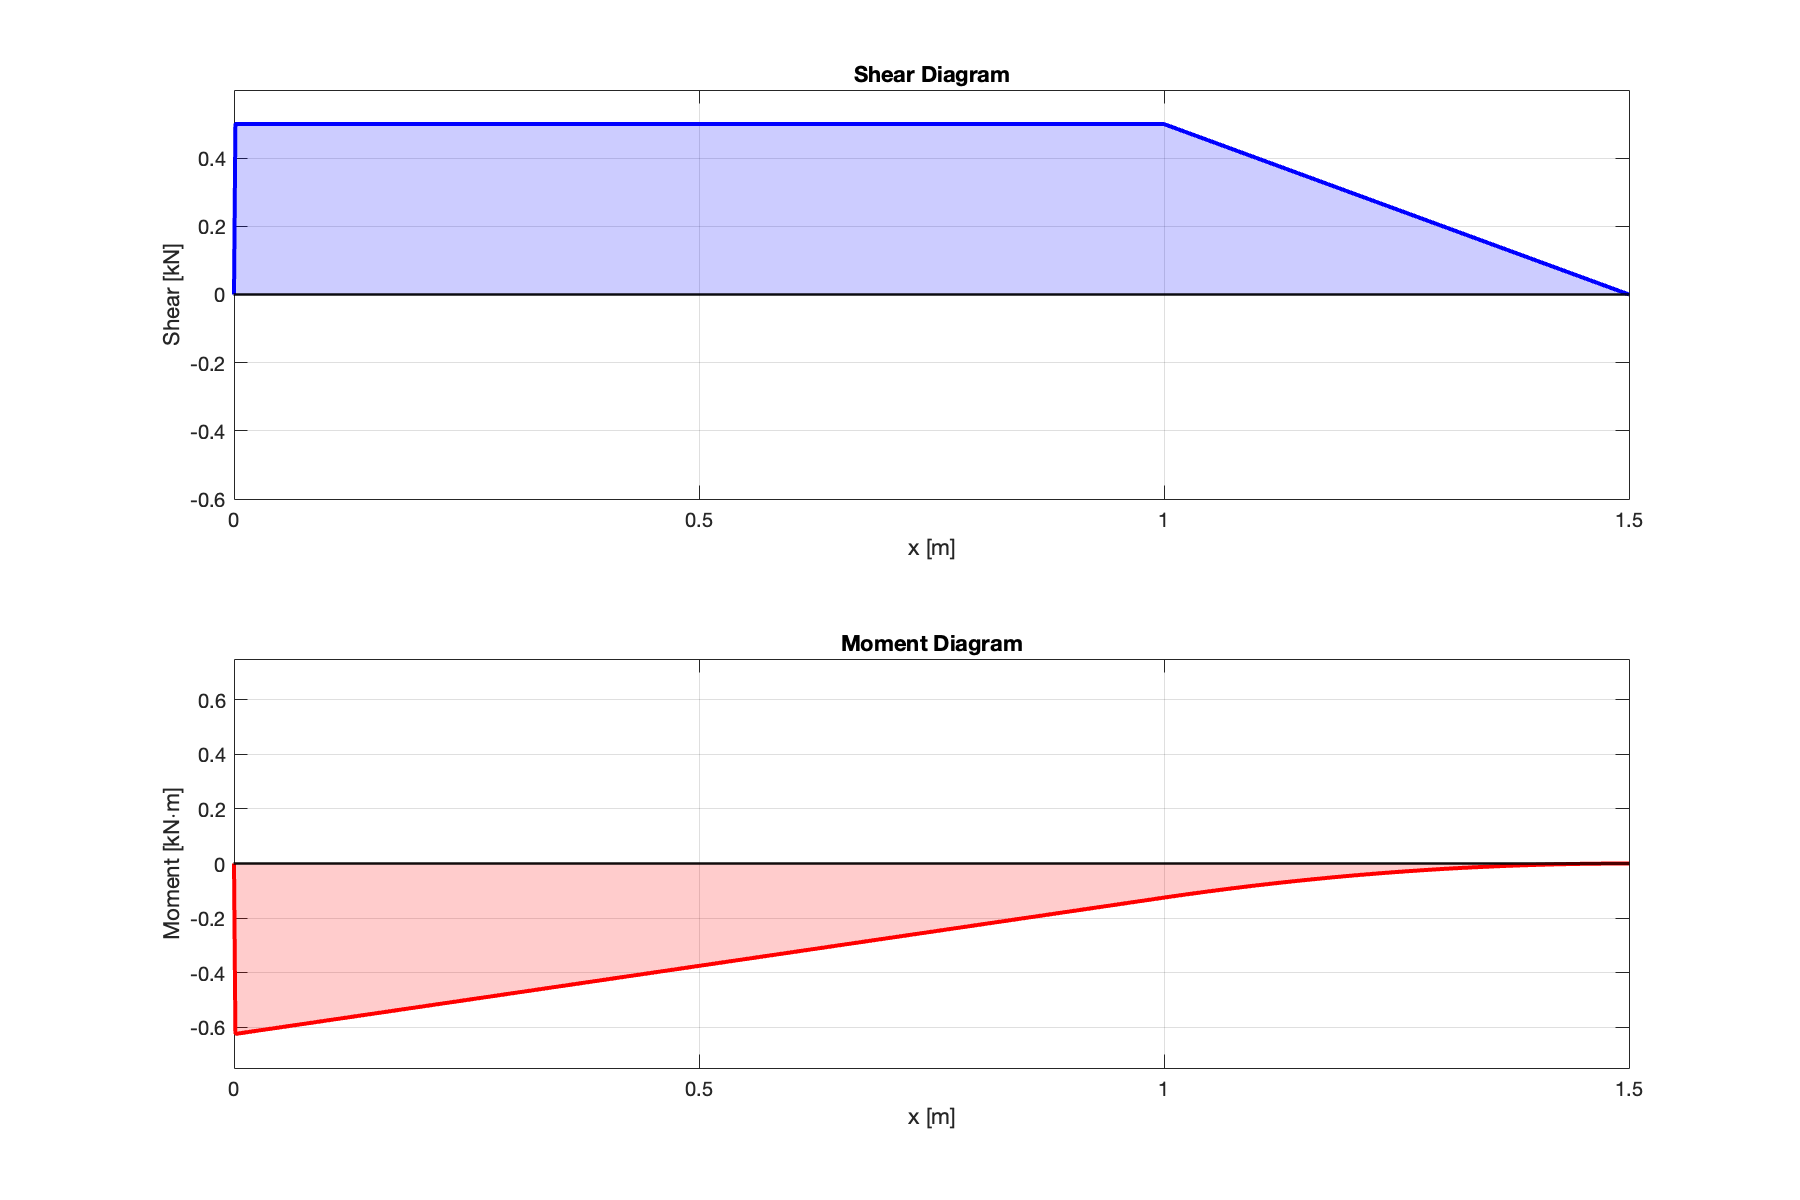
\includegraphics[width=0.8\linewidth]{./figures/e2025r2sm.png}
        \caption{Shear and moment diagram.}
        \label{fig:e2025r2sm}
      \end{figure}
      
    \item[Q2.3] For an Euler-Bernoulli beam, we have that
      \begin{equation*}
        EI v''(x) = M(x)
      .\end{equation*}
      Which will be integrated piecewise.
      For $0 < x < L$ we get
      \begin{align*}
        v_1''(x) &= - \frac{q L}{2} \left( \frac{5}{4}L - x \right) \cdot \frac{1}{E I} \\
        v_1'(x) &=  -\frac{L q \left(5 L x-2 x^2\right)}{8 EI} + C_1 \\
        v_1(x) &= -\frac{L q x^2 (15 L-4 x)}{48 EI} + C_1 x + C_2
      .\end{align*}
      Here we use that $v(0) = 0 \implies C_2 = 0$ and as rotation if prevented $v'(0) = 0 \implies C_1 = 0$ so
      \begin{equation*}
        v_1(x) = - \frac{L q x^2 \left( 15 L - 4 x \right)}{48 EI}, \quad 0 < x < L
      .\end{equation*}
      
      And for $L < x < 3 / 2 L$ we get
      \begin{align*}
        v_2''(x) &= - \frac{q}{2} \left( \frac{3}{2} L - x \right)^2 \cdot \frac{1}{EI}\\
        v_2'(x) &= \frac{q (3 L-2 x)^3}{48 EI} + C_3 \\
        v_2(x) &= -\frac{q (3 L-2 x)^4}{384 EI} + C_3 x + C_4
      .\end{align*}
      
      For continuity at $x = L$ we require $v_1(L) = v_2(L)$ and $v_1'(L) = v_2'(L)$, so,
      \begin{align*}
        v_1(L) &= v_2(L) \\
        v_1'(L) &= v_2'(L) \\
        - \frac{L q L^2 \left( 15 L - 4 L \right)}{48 EI} &= - \frac{q \left( 3 L - 2 L \right)^{4}}{384 EI} + C_3 L + C_4 \\
        - \frac{L q \left( 5 L^2 - 2 L^2 \right)}{8 EI} &= \frac{q \left( 3 L - 2 L \right)^3}{48 EI} + C_3 \\
        C_3 &\to -\frac{19 L^3 q}{48 EI} \\
        C_4 &\to \frac{65 L^4 q}{384 EI}.
    \end{align*}
    So
    \begin{equation*}
      v(x) = \begin{cases}
        - \frac{L q x^2 (15 L - 4x)}{48EI} & 0 \leq x \leq L\\
      - \frac{q (3L - 2x)^{4}}{348 EI} - \frac{19 q L^3}{48EI} x + \frac{65 L^{4} q }{384EI} & L \leq x \leq \frac{3}{2}L
      .\end{cases}
    .\end{equation*}
    This is plotted on \Cref{fig:e2025r2d}.

    \begin{figure} [ht]
      \centering
      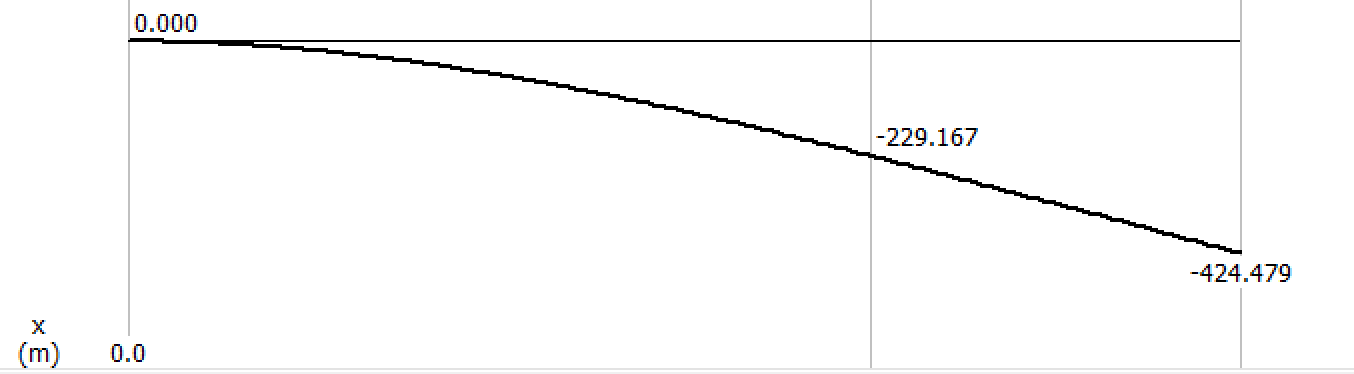
\includegraphics[width=0.8\linewidth]{./figures/e2025r2d.png}
      \caption{Deflection of the beam.}
      \label{fig:e2025r2d}
    \end{figure}
    The maximum deflection happens at the beam tip, where the deflection is:
    \begin{align*}
      v \left( \frac{3}{2}L \right) &= - \frac{q (3L - 2 \cdot \frac{3}{2} L)^{4}}{384 EI} - \frac{19qL^3}{48EI} \cdot \frac{3}{2}L + \frac{65 L^{4} q}{384 EI} \\
      &= - \frac{57 q L^4}{96 EI} + \frac{65 L^{4} q}{384 EI} \\
      &= -\frac{163 L^4 q}{384 EI}
    .\end{align*}
    
  \item[Q2.4] The resultants at the fixed end are, as derived above:
    \begin{equation*}
      R_y =  \frac{qL}{2}, \qquad M_0 = - \frac{qL}{2} \cdot \frac{5}{4} L = - \frac{5 q L^2}{8}
    .\end{equation*}
    We, furthermore, know that
    \begin{equation*}
      \sigma_x = - \frac{M(x) y}{I}
    \end{equation*}
    and
    \begin{equation*}
      \tau = \frac{V(x) Q(y)}{I t}
    .\end{equation*}
    The second moment of area $I$ of the rectangular cross section is
    \begin{equation*}
      I = \frac{bh^3}{12} = \frac{\qty{50}{\mm} \cdot \left( \qty{100}{\mm}  \right)^3}{12} = \qty{4,1667e6}{\mm^{4}} 
    .\end{equation*}
    For the top fibre we get:
    \begin{align*}
      \sigma_{\mathrm{top}} &= -\frac{M_0 \cdot \frac{h}{2}}{I} \\
      &= \frac{5 L^2 h}{16 \cdot I} q \\
      &=  \frac{5 \cdot \left( \qty{1.5}{\m}  \right)^2 \cdot \qty{100}{\mm} }{16 \cdot \qty{4.1667e6}{\mm^{4}} } q\\
      &= \qty{16,874e3}{\m^{-1}} q
    .\end{align*}
    and
    \begin{align*}
      \tau_{\mathrm{top}} &= \frac{V(x) Q(y)}{I t} \\
      &= - \frac{L \cdot Q}{2 I} q\\
      &= - \frac{\qty{1.5}{\m} \cdot \qty{0}{\mm^3}  }{2 \cdot \qty{4,1667e6}{\mm^{4}} } \\
      &=  0
    .\end{align*}

    For the bottom fibre ($x = 0$, $y = - h / 2$ we get
    \begin{align*}
      \sigma_{\mathrm{bot}} &= \frac{M_0 h}{2I} \\
      &= - \frac{5 L^2 h}{16 I} q \\
      &= - \qty{16,874e3}{\m^{-1}} q
    .\end{align*}
    and
    \begin{align*}
      \tau_{\mathrm{bot}} &= \frac{- \frac{5}{8} qL^2 \cdot \qty{0}{\mm^3}}{I b} \\
      &= 0
    .\end{align*}

    For the fibre at the neutral axis we get:
    \begin{align*}
      \sigma_{NA} &= - \frac{M(x) y}{I} \\
      &= \frac{M(x) \cdot \qty{0}{\mm} }{I} \\
      &= 0
    .\end{align*}
    and
    \begin{align*}
      \tau_{NA} &= \frac{V(x) Q(y)}{I t} \\
      &= -\frac{qL}{2} \cdot \frac{bh}{2} \cdot \frac{h}{4} \cdot \frac{1}{Ib} \\
      &= \frac{L h^2}{16 I} q\\
      &= \frac{\qty{1.5}{\m} \cdot \left( \qty{100}{\mm}  \right)^2}{16 \cdot \qty{4,1667e6}{\mm^{4}} } \\
      &= \qty{225}{\m^{-1}} q
    .\end{align*}

  \item[Q2.5] At the top fibre we have:
    \begin{equation*}
      \sigma_x = \qty{16,874e3}{\m^{-1}} q \qquad \sigma_y = 0 \qquad \tau_{xy} = 0
    .\end{equation*}

    The Mohr's circle is thus given by
    \begin{align*}
      \sigma_{\mathrm{avg}} &= \frac{\sigma_x + \sigma_y}{2} = \frac{\qty{16,874e3}{\m^{-1}} q}{2} = \qty{8,437e3}{\m^{-1}} q \\
      R &= \sqrt{\left( \frac{\sigma_x - \sigma_y}{2}\right)^2 + \tau_{xy}^2} = \sqrt{\left( \frac{\qty{16.874e3}{\m^{-1}} q}{2} \right)^2} = \qty{8,437e3}{\m^{-1}} q
    .\end{align*}
    The principal stresses are given by:
    \begin{equation*}
      \sigma_{1,2} = \sigma_{\mathrm{avg}} \pm R \implies \sigma_1 = \sigma_x, \sigma_2 = 0
    .\end{equation*}
    This circle is shown on \Cref{fig:e2025r2m}.

    \begin{figure} [ht]
      \centering
      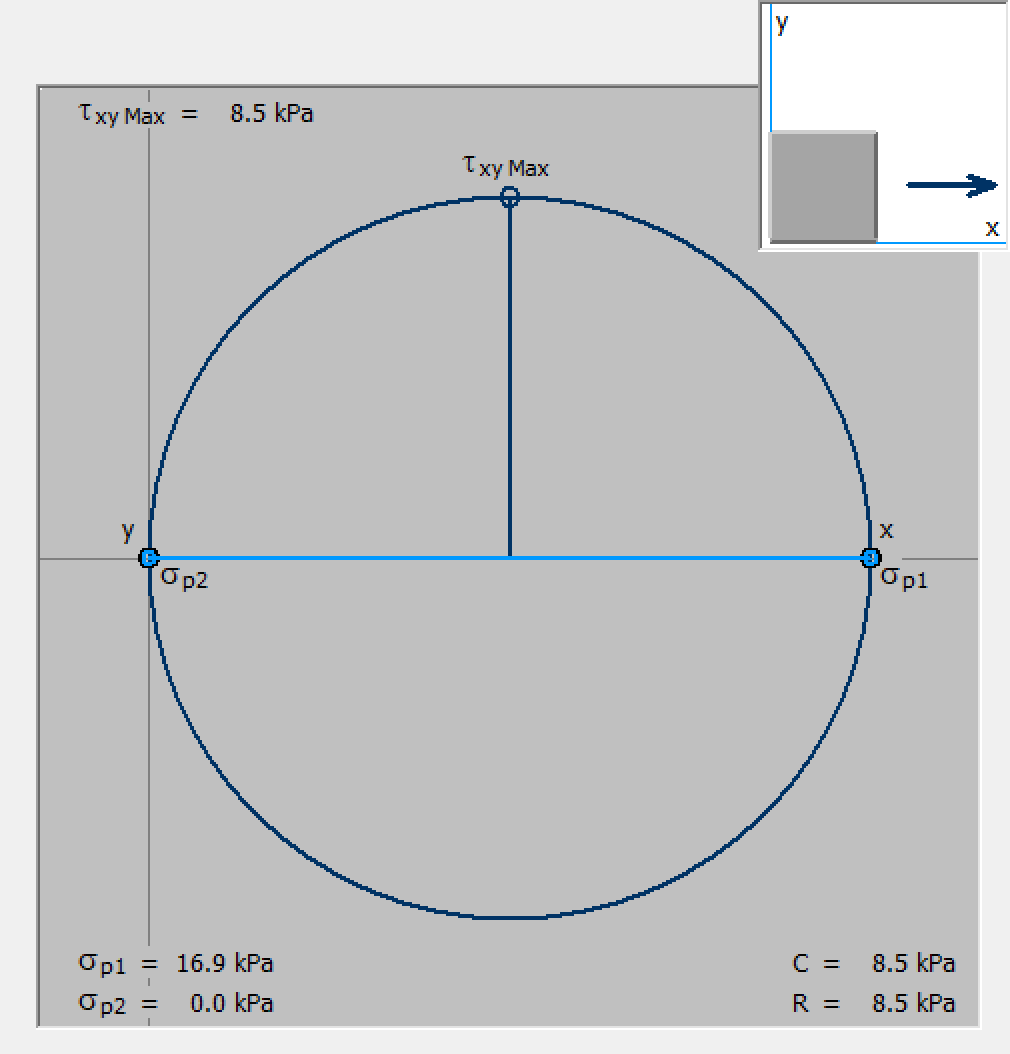
\includegraphics[width=0.5\linewidth]{./figures/e2025r2m.png}
      \caption{Mohr's circle for the stress state at the top-fibre.}
      \label{fig:e2025r2m}
    \end{figure}
  \end{itemize}
\end{derivation}

\finalresult{
\begin{aligned}
  &\mathrm{Q2.1} & &\text{See the section}\\
  &\mathrm{Q2.2} & &\text{See \Cref{fig:e2025r2sm}} \\
  &\mathrm{Q2.3} & &\text{See \Cref{fig:e2025r2d}} \\
  && v \left( \frac{3}{2}L \right) &= - \frac{163}{384 EI} L^{4}q \\
  &\mathrm{Q2.4} & \sigma_{\mathrm{top}} &= \qty{16,874e3}{\m^{-1}} q \\
  && \tau_{\mathrm{top}} &= 0 \\
  && \sigma_{\mathrm{bot}} &= - \qty{16,874e3}{\m^{-1}} q\\
  && \tau_{\mathrm{bot}} &= 0 \\
  && \sigma_{NA} &= 0 \\
  && \tau_{NA} &= \qty{225}{\m^{-1}} q \\
  &\mathrm{Q2.5} & \sigma_1 &= \sigma_x \\
  && \sigma_2 &= 0 \\
  && &\text{See \Cref{fig:e2025r2m}}
.\end{aligned}
}
